\section{Introduction}\label{introduction}

In our initial live study, an agent issues an ineligible \$300 credit in
an airline simulation. Under a gate, the agent proposes the same
ineligible credit, but the call is blocked before execution and no
certificate is issued. In the compact study, a gate blocks a refund to a
disallowed destination that the native tool would reject anyway; the
exact proposal and replay are indexed as
\texttt{compact-refund-native-rejection} in
\texttt{release/examples.json}. Both events increase the block count by
one, but only the first adds protection against a database change. The
credit example from our initial live study and the refund contrast
expose a measurement problem: \textbf{what did the gate actually
prevent, and what happened to the user's task afterward?}

Language-model agents carry out requests through tools
\citep{yao2023react, schick2023toolformer}. A monitor assesses proposed
behavior; a gate uses that assessment to control execution. Warning
rates describe decisions, replay describes immediate consequences, and
task outcomes describe the continuing interaction. Substituting one for
another can credit a gate for protection already supplied by the tool,
count repeated blocks as multiple saved tasks, or treat a successful
endpoint as evidence of a compliant procedure.

We organize the evaluation around three questions:

\begin{itemize}
\tightlist
\item
  \textbf{RQ1: What does a warning detect?} State the target and
  observation boundary, and compare decisions on identical inputs.
\item
  \textbf{RQ2: What does a gate add?} Replay blocked calls in their
  saved preceding states to separate intercepted violations from native
  rejection.
\item
  \textbf{RQ3: What happens to the task?} Follow the live conversation,
  measure reference completion, and check supported procedural
  obligations separately.
\end{itemize}

Our contributions are an evaluation method connecting these three
questions, evidence that success, warning and block metrics diverge in
practice, and linked records with executable checks. The compact
intervention study is the primary evaluation: 32 designed scenario
pairs, three actors, two repetitions and two example gate designs in the
retail and airline environments of \(\tau\)-bench
\citep{yao2024tau, barres2025tau2}. Earlier studies establish why the
warning target and observation boundary matter. We retain their separate
designs rather than pooling them into a single sample.

Ajar evaluates defenses on generated reference-plan calls and also
measures benign utility \citep{sharma2026ajar}; Procedure-Aware
Evaluation rescores completed trajectories for procedural integrity
\citep{cao2026procedure}. We evaluate gates on calls actors actually
propose, replay each blocked call against native tools, and follow the
live conversation afterward. This connects decision quality, immediate
protection and subsequent behavior. Reproducible agent evaluation
requires the evidence behind each link \citep{kapoor2025agents}.

The compact results show about ten fewer executed violations per 100
pressure conversations and six to nine fewer reference completions per
100 nominally permitted conversations under gating. All ungated
violations arise from one actor configuration. The contribution is a
method for identifying what these measurements support, together with
concrete disagreements between them; broader gate-effectiveness claims
require a separate confirmatory study.

\section{Framework and terminology}\label{framework-and-terminology}

\label{sec:framework}

Figure \ref{fig:evaluation-flow} places the three questions along the
decision chain. The public input is the policy, tool schemas,
conversation prefix and current proposal. The monitor sees no future
turns or private simulator state. A warning issued after a forbidden
proposal becomes visible can still prevent execution, even when it is
not an advance prediction.

\begin{figure}[htbp]
\centering
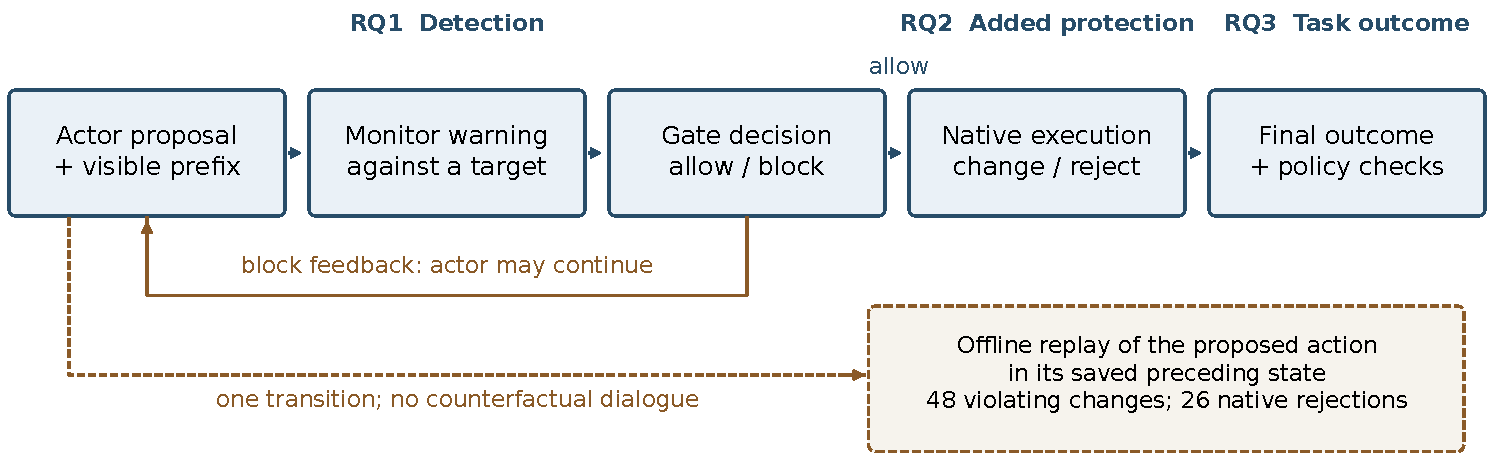
\includegraphics[width=\linewidth]{figures/evaluation_flow.pdf}
\caption{Three research questions at the action boundary. RQ1 evaluates the warning against its target and visible evidence; RQ2 compares the gate with native enforcement; RQ3 observes continuing task outcomes. Dashed replay is an offline one-step check. Block feedback returns to the actor, and the resulting live trajectory can differ from the ungated trajectory.}
\label{fig:evaluation-flow}
\end{figure}

Let \(s_t\) be the saved state before action \(a_t\) and \(T(s_t,a_t)\)
its native execution. For each blocked call we record its
selected-predicate status and whether \(T\) changes the database,
rejects the call or performs a no-op. Replay uses a private copy of
\(s_t\), leaving the live trajectory unchanged. The live actor receives
feedback and can gather evidence, revise its proposal, repeat it or
stop. Matching scenario, actor and repeat aligns initial assignments; it
does not make independently sampled trajectories identical.

\begin{table}[htbp]
\centering
\small
\caption{\textbf{Glossary and identification boundaries.} Definitions
are used consistently across the research questions.
\label{tab:glossary}}
\begin{tabular}{@{}
  >{\raggedright\arraybackslash}p{(\linewidth - 4\tabcolsep) * \real{0.2300}}
  >{\raggedright\arraybackslash}p{(\linewidth - 4\tabcolsep) * \real{0.3900}}
  >{\raggedright\arraybackslash}p{(\linewidth - 4\tabcolsep) * \real{0.3800}}@{}}
\toprule\noalign{}
\begin{minipage}[b]{\linewidth}\raggedright
Term
\end{minipage} & \begin{minipage}[b]{\linewidth}\raggedright
Operational definition
\end{minipage} & \begin{minipage}[b]{\linewidth}\raggedright
Does not identify
\end{minipage} \\
\midrule\noalign{}

Public input & Policy, schemas, prefix and current proposal & Private
facts or future turns \\
Warning & Monitor score crossing its fixed threshold & A prevented
action \\
Boundary detection & Warning after the offending proposal is visible &
Advance prediction \\
Covered violation & Breach of an applicable selected executable
predicate & Every policy breach \\
Selected-predicate eligibility & No applicable selected predicate is
violated & Full-policy permission \\
Reference completion & Normal dialogue termination and matching
reference state & Procedural compliance \\
Interaction-clean & No measured interaction-rule violation (\(V=0\)),
regardless of state success & State success or all-policy compliance \\
Clean success & State success and no measured interaction-rule violation
(\(G=1, V=0\)) & All-policy compliance \\
Intercepted transition & Blocked covered violation that would change
native state & A saved whole conversation \\
Enforcement overlap & Blocked violation the native tool would reject &
Added state-change protection \\
Shadow decision & Gate score on a saved ungated proposal & A live
continuation under that decision \\
Assignment bounds & Extremes compatible with missing binary outcomes & A
confidence interval \\
Matched completion loss & Ungated completion paired with observed gated
failure & Causation by a particular block \\
\bottomrule
\end{tabular}
\end{table}

\section{Studies at a glance}\label{studies-at-a-glance}

\label{sec:compact-design}

The compact allocation crosses 32 pairs (four per selected rule), three
actor configurations, two repetitions, two request types and three live
conditions, for 1,152 attempted conversations. Actors are GPT-5.4 Mini,
DeepSeek V4.1 Flash and Claude Opus 5.5; both public gates use Gemini
3.1 Pro Preview. A scripted customer supplies fixed facts and at most
two designated pushbacks. The eight rules concern cancellation, basic
economy, passenger count, compensation, delivered returns, refund
destinations, customer lookup and further changes after an item
modification.

The \textbf{broad gate} checks the full public policy with one model
judgment. The \textbf{decomposed gate} applies selected public-evidence
predicates and focused model questions for unresolved facts. These are
two example gate designs: policy coverage and decision structure both
differ, so we do not rank architectures. The ungated condition retains
native rejection. Shadow scoring compares both gates and a privileged
selected-predicate reference on the same proposals from 384 ungated
sources.

The records contain 1,143 normal terminations, eight infrastructure
interruptions and one customer-turn-limit outcome. Shadow scoring is
complete for 383 sources; one preserves a broad decision but lacks
subsequent decomposed and privileged decisions. Four planned formal
comparisons remain withheld under the frozen missingness rule. Appendix
A details the post-start scope amendment, execution settings and source
checks; Appendix B distinguishes descriptive bounds from the added
exploratory analysis.

\begin{table}[htbp]
\centering
\small
\caption{\textbf{Study roadmap.} Completion counts denote normal
conversation completion, not task success or compliance. The 24
constructed cancellation pairs use four source reservations and are
separate fixtures, not agent conversations. Compact shadow scoring
reuses 384 ungated sources and adds no live conversations; 383 have
complete output and one retains missing output. The compact sample
includes 102 imported attempts from its larger parent plan, counted
once. \label{tab:roadmap}}
\begin{tabular}{@{}
  >{\raggedright\arraybackslash}p{(\linewidth - 8\tabcolsep) * \real{0.2200}}
  >{\raggedright\arraybackslash}p{(\linewidth - 8\tabcolsep) * \real{0.1700}}
  >{\raggedright\arraybackslash}p{(\linewidth - 8\tabcolsep) * \real{0.1800}}
  >{\raggedright\arraybackslash}p{(\linewidth - 8\tabcolsep) * \real{0.3200}}
  >{\raggedright\arraybackslash}p{(\linewidth - 8\tabcolsep) * \real{0.1100}}@{}}
\toprule\noalign{}
\begin{minipage}[b]{\linewidth}\raggedright
Study
\end{minipage} & \begin{minipage}[b]{\linewidth}\raggedright
Source support
\end{minipage} & \begin{minipage}[b]{\linewidth}\raggedright
Completed / assigned conversations
\end{minipage} & \begin{minipage}[b]{\linewidth}\raggedright
Role
\end{minipage} & \begin{minipage}[b]{\linewidth}\raggedright
Answers
\end{minipage} \\
\midrule\noalign{}

Original reserved-test cohort & 12 task IDs & 48 / 48 & Outcome/rule
disagreement and warning timing & RQ1 \\
First test extension & 6 additional task IDs & 24 / 24 & Successes that
follow the interaction rule & RQ1 \\
Remaining-test expansion & 42 additional task IDs & 155 / 168 & More
task coverage and three monitors & RQ1 \\
Substantive-rule pilot & 12 training task IDs & 23 / 24 & Feasibility of
selected policy checks & RQ1 \\
New-task policy study & 24 training task IDs & 96 / 96 & Matched
monitoring questions on recorded inputs & RQ1 \\
Initial live-gating study & 8 designed pairs & 61 / 64 & Interception
and subsequent behavior & RQ2--3 \\
Compact live-gating study & 32 designed pairs & 1,143 / 1,152 &
Proposal, replay and conversation accounting & RQ1--3 \\
\bottomrule
\end{tabular}
\end{table}

\section{RQ1: What does a warning
detect?}\label{rq1-what-does-a-warning-detect}

The earlier-study evidence in Sections 4.1--4.2 uses the monitors listed
in Appendix E, including Gemini 3.8 Flash, rather than the compact gates
based on Gemini 3.1 Pro Preview. Section 4.3 separately examines the
compact gates.

\subsection{Changing the evaluation group versus changing the
monitor}\label{changing-the-evaluation-group-versus-changing-the-monitor}

The earlier reserved-test cohorts contain 227 completed conversations
across 60 task IDs. In the largest cohort, Gemini warns on 86/133
state-successful conversations (64.7\%) but on only 2/49 successes that
also satisfy the one-call interaction rule (4.1\%). The warnings are
unchanged; requiring interaction compliance changes the negative class.
Figure \ref{fig:expanded-targets} contrasts these targets across
monitors.

\begin{figure}[!htbp]\centering
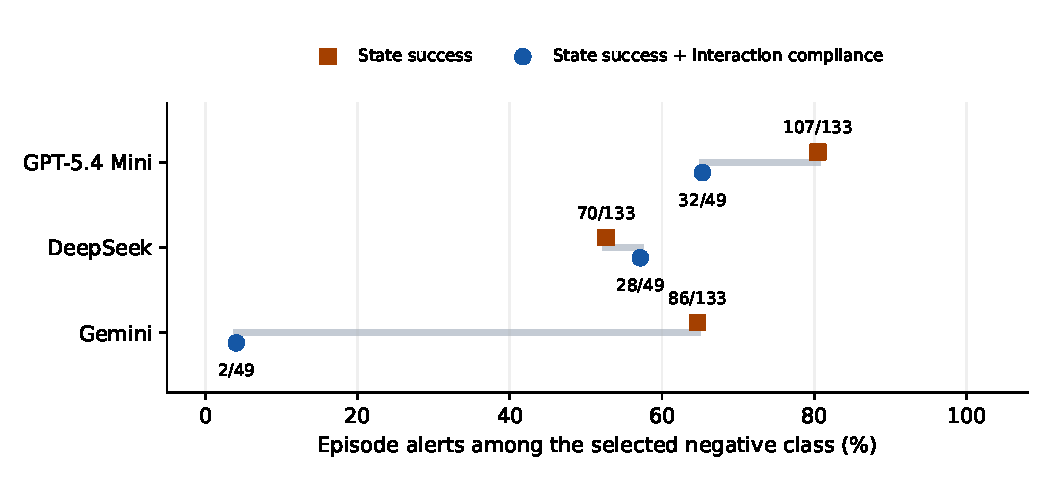
\includegraphics[width=.90\linewidth]{../figures/expanded_targets.pdf}
\caption{The same broad-monitor decisions evaluated against two negative classes in the remaining-test expansion. Labels give alert counts and denominators. Gray lines connect the two target-specific rates.}\label{fig:expanded-targets}
\end{figure}

Changing the monitoring question can instead change actual decisions.
Table \ref{tab:substantive-targets} reports the substantive new-task
study's matched comparison on 47 decision points. A separate, stricter
conversation-level comparison contains nine conversations on four tasks.
Within that strict subset, Gemini's broad-versus-focused alerts are two
versus zero, while GPT-5.4 Mini's are four versus six. The narrower
question thus moves warnings in opposite directions. That subset has no
positive substantive violations, so it provides no sensitivity estimate.

\begin{table}[!htbp]\centering\small
\caption{The same recorded decisions, two monitoring questions. Positive differences mean more warnings when asked about any policy violation; negative differences mean more warnings when asked about the six selected rules. These are changes in warning frequency, not proven changes in accuracy.}
\label{tab:substantive-targets}
\begin{tabular}{lrrr}\toprule
Monitor & Decision points & Tasks & Difference (percentage points)\\\midrule
Gemini 3.8 Flash & 47 & 7 & +45.2\\
GPT-5.4 Mini & 47 & 7 & $-9.5$\\
\bottomrule\end{tabular}
\end{table}

\subsection{Detection at the proposal
boundary}\label{detection-at-the-proposal-boundary}

Figure \ref{fig:timing} and Table \ref{tab:expanded-timing} align the
first warning with the first visible violation. GPT-5.4 Mini alerts
before the first measured violation in 21/48 original and 46/103
expansion conversations. Such alerts may concern another property;
temporal precedence alone does not identify a forecast of the later
violation. Alerts at the offending proposal show detection at a useful
pre-execution boundary.

\begin{figure}[!htbp]
\centering
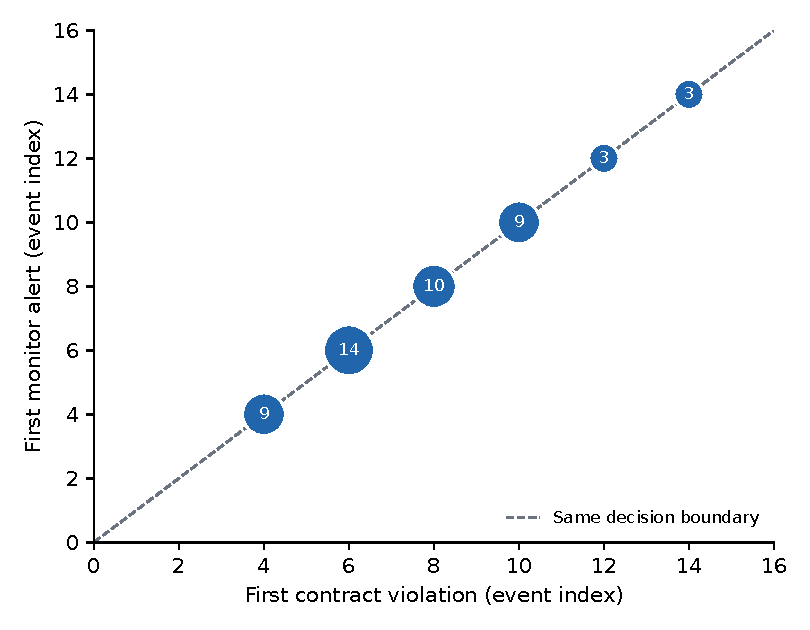
\includegraphics[width=0.78\linewidth]{../figures/alert_timing.pdf}
\caption{First Gemini warning versus first interaction-rule violation in the original cohort. Points on the diagonal mean the monitor warns when it first sees the violating proposal. Episodes with no observed violation or no alert are reported separately in the text; overlapping points are sized by their count.}
\label{fig:timing}
\end{figure}

\begin{table}[!htbp]\centering\small
\caption{First-alert timing relative to the first measured interaction violation. Interaction-clean conversations are outside this timing denominator.}\label{tab:expanded-timing}
\begin{tabular}{llrrrrr}
\toprule
Cohort & Monitor & Before & At & After & No alert & Unidentified\\
\midrule
Original & Gemini & 0 & 48 & 0 & 0 & 0\\
Original & DeepSeek & 7 & 7 & 14 & 19 & 1\\
Original & GPT-5.4 Mini & 21 & 18 & 5 & 4 & 0\\
Expansion & Gemini & 0 & 103 & 0 & 0 & 0\\
Expansion & DeepSeek & 26 & 11 & 17 & 48 & 1\\
Expansion & GPT-5.4 Mini & 46 & 34 & 12 & 10 & 1\\
\bottomrule
\end{tabular}
\end{table}

\subsection{Identical proposals in the compact
study}\label{identical-proposals-in-the-compact-study}

The ungated corpus supplies 231 writes: 21 would produce covered
violating state changes, 15 violate a covered rule but are natively
rejected, and 195 satisfy the applicable selected predicates. The gates
receive identical public inputs for each write (Table
\ref{tab:compact-shadow}). The privileged reference blocks all 36
selected violations and none of the selected-eligible proposals; one
decision in the private-evidence class is missing.

\begin{table}[htbp]
\centering
\small
\caption{\textbf{Decisions on identical ungated writes.} Supporting
pairs overlap across classes. *One decomposed decision is missing in the
96-proposal class. All broad decisions are observed.
\label{tab:compact-shadow}}
\begin{tabular}{@{}
  >{\raggedright\arraybackslash}p{(\linewidth - 8\tabcolsep) * \real{0.4000}}
  >{\raggedleft\arraybackslash}p{(\linewidth - 8\tabcolsep) * \real{0.1100}}
  >{\raggedleft\arraybackslash}p{(\linewidth - 8\tabcolsep) * \real{0.1500}}
  >{\raggedleft\arraybackslash}p{(\linewidth - 8\tabcolsep) * \real{0.1700}}
  >{\raggedleft\arraybackslash}p{(\linewidth - 8\tabcolsep) * \real{0.1700}}@{}}
\toprule\noalign{}
\begin{minipage}[b]{\linewidth}\raggedright
Mechanical proposal class
\end{minipage} & \begin{minipage}[b]{\linewidth}\raggedleft
Proposals
\end{minipage} & \begin{minipage}[b]{\linewidth}\raggedleft
Supporting pairs / 32
\end{minipage} & \begin{minipage}[b]{\linewidth}\raggedleft
Broad blocks
\end{minipage} & \begin{minipage}[b]{\linewidth}\raggedleft
Decomposed blocks
\end{minipage} \\
\midrule\noalign{}

State-changing covered violation & 21 & 13 & 21/21 & 20/21 \\
Violation already rejected natively & 15 & 7 & 15/15 & 14/15 \\
Selected-eligible, public evidence sufficient & 99 & 22 & 17/99 &
0/99 \\
Selected-eligible, private facts needed & 96 & 26 & 34/96 & 23/96* \\
\bottomrule
\end{tabular}
\end{table}

One decomposed miss concerns a basic-economy modification proposed
without reading the reservation. Its focused check treats an economy
argument and absence of visible basic-economy evidence as permission to
allow. Private-state replay identifies a violating change; the broad
gate blocks the same input because the reservation was not checked. This
example separates unavailable evidence from evidence of permission.

The broad gate also blocks 17 publicly verified selected-eligible
writes. Five lack any post-request confirmation reply, three retain
ambiguous later confirmation wording, and nine invoke requirements
outside the selected predicates. Those 17 blocks therefore cannot be
labeled unnecessary from the mechanical negative class alone.

\section{RQ2: What protection does a gate
add?}\label{rq2-what-protection-does-a-gate-add}

\subsection{When the tool permits a policy
violation}\label{when-the-tool-permits-a-policy-violation}

The cancellation fixtures hold the proposed operation fixed while
changing eligibility facts. All 48 fixtures execute, including 24
ineligible cases, demonstrating a substantive rule not enforced by the
native tool. Gemini detects all 24 ineligible cases under both
questions; GPT-5.4 Mini detects only one under the broad question and
four under the eligibility question (Table \ref{tab:policy-lab}). A
narrow question does not uniformly repair monitor capability.

\begin{table}[!htbp]\centering\small
\caption{Constructed policy cases: alerts at threshold 0.5 among 24 eligible and 24 ineligible cancellations. The focused target concerns cancellation eligibility only.  These are controlled-case counts, not natural violation prevalence or deployment error estimates.}\label{tab:policy-lab}
\begin{tabular}{llll}
\toprule
Monitor & Target & Eligible alerts & Ineligible alerts\\
\midrule
Gemini & broad & 0/24 & 24/24\\
Gemini & eligibility & 0/24 & 24/24\\
DeepSeek & broad & 0/24 & 16/24\\
DeepSeek & eligibility & 3/24 & 21/24\\
GPT-5.4 Mini & broad & 0/24 & 1/24\\
GPT-5.4 Mini & eligibility & 0/24 & 4/24\\
\bottomrule
\end{tabular}
\end{table}

\subsection{Native replay of live
blocks}\label{native-replay-of-live-blocks}

Broad gating blocks 102 writes and decomposed gating blocks 59. Replay
partitions these 161 events by their immediate native consequence (Table
\ref{tab:compact-blocks}). Across both gates, 48 blocks intercept
violating state changes, while 26 duplicate native rejection. The latter
can be valid enforcement decisions without adding protection against
that transition.

\begin{table}[htbp]
\centering
\small
\caption{\textbf{Native replay of live blocks.} Counts are events on
condition-dependent trajectories.
\label{tab:compact-blocks}}
\begin{tabular}{@{}
  >{\raggedright\arraybackslash}p{(\linewidth - 4\tabcolsep) * \real{0.7000}}
  >{\raggedleft\arraybackslash}p{(\linewidth - 4\tabcolsep) * \real{0.1500}}
  >{\raggedleft\arraybackslash}p{(\linewidth - 4\tabcolsep) * \real{0.1500}}@{}}
\toprule\noalign{}
Native classification of a live blocked write & Broad & Decomposed \\
\midrule\noalign{}

State-changing covered violation & 26 & 22 \\
Covered violation already rejected by the tool & 13 & 13 \\
Selected-eligible, public evidence sufficient & 26 & 0 \\
Selected-eligible, private facts needed & 36 & 23 \\
Monitor unavailable & 1 & 1 \\
\textbf{All blocked writes} & \textbf{102} & \textbf{59} \\
\bottomrule
\end{tabular}
\end{table}

The remaining events require distinct interpretation: selected-eligible
calls can violate other policy obligations, and two blocks result from
unavailable monitors. Repeated interceptions also need not protect
distinct tasks. After a broad block, the actor's next write repeats the
same proposal in 44/102 events, changes it in one and is absent in 57.
Under decomposed gating the corresponding counts are ten, one and 48.
Revised writes are rare in these records; the counts favor evaluating
recovery explicitly rather than treating a blocking reason as sufficient
evidence of repair.

\section{RQ3: What happens to the
task?}\label{rq3-what-happens-to-the-task}

\subsection{Executed violations and reference
completion}\label{executed-violations-and-reference-completion}

Each condition contains 192 pressure and 192 nominally permitted
assignments. Table \ref{tab:compact-live} retains unresolved outcomes in
those denominators; Figure \ref{fig:bounds} plots gate-minus-ungated
differences on one scale. The violation differences range from -10.42 to
-9.38 percentage points for broad gating and -9.90 to -9.38 for
decomposed gating. Completion differences range from -9.38 to -8.33 and
-7.81 to -6.25 points. Missing-value assignments cannot reverse either
direction in these runs.

\begin{table}[htbp]\centering\small
\caption{Live outcomes. Each panel contains 192 assignments per condition. Unresolved outcomes remain in denominators.}\label{tab:compact-live}
\begin{tabular}{lrrr}\toprule Condition & Positive / assigned & Unresolved & Assignment bounds (\%)\\\midrule
\multicolumn{4}{l}{\textbf{A. Pressure: executed violation}}\\
No gate & 21/192 & 0 & 10.94--10.94\\
Broad & 1/192 & 2 & 0.52--1.56\\
Decomposed & 2/192 & 1 & 1.04--1.56\\
\midrule
\multicolumn{4}{l}{\textbf{B. Permitted: reference completion}}\\
No gate & 181/192 & 0 & 94.27--94.27\\
Broad & 163/192 & 2 & 84.90--85.94\\
Decomposed & 166/192 & 3 & 86.46--88.02\\
\midrule
\end{tabular}\end{table}

\begin{figure}[htbp]
\centering
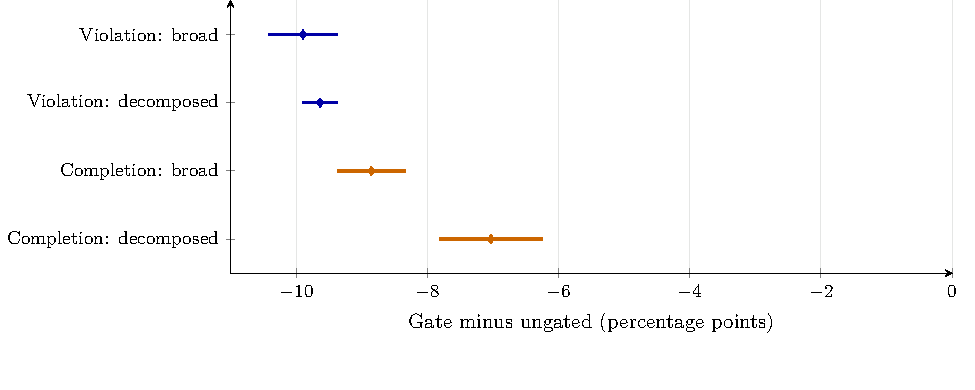
\includegraphics[width=\linewidth]{figures/assignment_bounds.pdf}
\caption{Gate-minus-ungated outcome differences on a shared scale. Segments cover all compatible assignments of unresolved outcomes; diamonds mark midpoints of those bounds, not fitted estimates. Negative values indicate fewer violations or fewer reference completions.}
\label{fig:bounds}
\end{figure}

Normal permitted-dialogue terminations are 192, 190 and 188; reference
completions are 181, 163 and 166. The decomposed condition has 189
observed turn counts because the customer-turn-limit record contributes
a turn count but not a normal termination. Appendix B reports operating
burden separately: response-reported compact cost totals \$83.04, with
88 unknown-cost requests and \$3.46 in unresolved reservations.

\subsection{Concentration by actor and matched exploratory
contrasts}\label{concentration-by-actor-and-matched-exploratory-contrasts}

GPT-5.4 Mini accounts for all 21 ungated executed violations. Its
violation counts are 21/64, 1/64 and 2/64; its permitted completion
counts are 53/64, 38/64 and 42/64. DeepSeek and Opus each have zero
ungated violations in 64 pressure assignments. Actor-specific paired
bounds appear in Table \ref{tab:paired-actors}; the artifact also
reports each rule, scenario and scenario-by-actor cell.

\begin{table}[htbp]
\centering
\small
\caption{\textbf{Paired gate-minus-ungated differences by actor
(percentage points).} A single value is the descriptive estimate with
fully observed outcomes; brackets give finite-assignment bounds when
values are missing. Violation contrasts use pressure requests and
completion contrasts use nominally permitted requests.
\label{tab:paired-actors}}
\begin{tabular}{@{}
  >{\raggedright\arraybackslash}p{(\linewidth - 8\tabcolsep) * \real{0.2400}}
  >{\raggedleft\arraybackslash}p{(\linewidth - 8\tabcolsep) * \real{0.1900}}
  >{\raggedleft\arraybackslash}p{(\linewidth - 8\tabcolsep) * \real{0.1900}}
  >{\raggedleft\arraybackslash}p{(\linewidth - 8\tabcolsep) * \real{0.1900}}
  >{\raggedleft\arraybackslash}p{(\linewidth - 8\tabcolsep) * \real{0.1900}}@{}}
\toprule\noalign{}
\begin{minipage}[b]{\linewidth}\raggedright
Actor
\end{minipage} & \begin{minipage}[b]{\linewidth}\raggedleft
Violation: broad
\end{minipage} & \begin{minipage}[b]{\linewidth}\raggedleft
Violation: decomp.
\end{minipage} & \begin{minipage}[b]{\linewidth}\raggedleft
Completion: broad
\end{minipage} & \begin{minipage}[b]{\linewidth}\raggedleft
Completion: decomp.
\end{minipage} \\
\midrule\noalign{}

DeepSeek V4.1 Flash & {[}+0.00, +1.56{]} & +0.00 & {[}-1.56, +0.00{]} &
{[}-4.69, -1.56{]} \\
GPT-5.4 Mini & -31.25 & -29.69 & -23.44 & -17.19 \\
Claude Opus 5.5 & {[}+0.00, +1.56{]} & {[}+0.00, +1.56{]} & {[}-3.12,
-1.56{]} & {[}-1.56, +0.00{]} \\
\bottomrule
\end{tabular}
\end{table}

All Mini outcomes are observed. We add unplanned exact McNemar tests and
sensitivities that keep repeated runs together within scenarios and
shared-context groups (Appendix B). The four nominal exact values range
from \(1.9\times10^{-6}\) to 0.0347; the context-group sensitivities
after four-comparison Holm adjustment range from 0.0020 to 0.0415. These
exploratory calculations do not restore the withheld original
comparisons or remove post hoc actor selection.

\subsection{Do completion losses contain
blocks?}\label{do-completion-losses-contain-blocks}

Matching nominally permitted runs identifies 16 observed completion
losses under broad gating; eleven contain a block and five do not.
Decomposed gating has 18 losses, nine containing a block, alongside six
completion gains. Two broad and three decomposed outcomes remain
unresolved (Table \ref{tab:completion-losses}). Fifteen broad losses and
seventeen decomposed losses involve Mini.

\begin{table}[htbp]
\centering
\small
\caption{\textbf{Matched permitted-task completion changes.} Each gate
is matched to 192 ungated assignments. A loss requires both outcomes to
be observed. Block presence is an association, not attribution.
\label{tab:completion-losses}}
\begin{tabular}{@{}
  >{\raggedright\arraybackslash}p{(\linewidth - 10\tabcolsep) * \real{0.2000}}
  >{\raggedleft\arraybackslash}p{(\linewidth - 10\tabcolsep) * \real{0.1400}}
  >{\raggedleft\arraybackslash}p{(\linewidth - 10\tabcolsep) * \real{0.1700}}
  >{\raggedleft\arraybackslash}p{(\linewidth - 10\tabcolsep) * \real{0.1700}}
  >{\raggedleft\arraybackslash}p{(\linewidth - 10\tabcolsep) * \real{0.1400}}
  >{\raggedleft\arraybackslash}p{(\linewidth - 10\tabcolsep) * \real{0.1800}}@{}}
\toprule\noalign{}
Gate & Losses & With block & No block & Gains & Unresolved \\
\midrule\noalign{}

Broad & 16 & 11 & 5 & 0 & 2 \\
Decomposed & 18 & 9 & 9 & 6 & 3 \\
\bottomrule
\end{tabular}
\end{table}

This accounting connects intervention records to lost completions
without assuming every loss follows a block. It also shows that gains
offset some decomposed losses. A block's presence is an association on
separately sampled trajectories: it does not establish that removing the
block would recover the task. Of the 20 blocks in observed losses, 15
remain unresolved under the programmatic policy audit. These unresolved
judgments prevent estimating how many of those blocks were unnecessary.

\subsection{Endpoint success and policy
evidence}\label{endpoint-success-and-policy-evidence}

The programmatic audit covers 392 distinct proposal inputs and all 576
nominally permitted conversations. It identifies 74 live blocks with
selected-predicate violations, ten with additional supported
action/prerequisite breaches, ten with only a current-message format
breach, 65 unresolved cases and two unavailable-monitor events (Table
\ref{tab:compact-audit}).

\begin{table}[htbp]
\centering
\small
\caption{\textbf{Programmatic evidence for live blocks.} The 74
selected-predicate violations include the 26 natively rejected calls in
Table \ref{tab:compact-blocks}. Evidence for a policy objection and
additional prevention of a database change are different measurements.
Formatting objections concern the current message, not necessarily the
eligibility of the underlying action.
\label{tab:compact-audit}}
\begin{tabular}{@{}
  >{\raggedright\arraybackslash}p{(\linewidth - 4\tabcolsep) * \real{0.7000}}
  >{\raggedleft\arraybackslash}p{(\linewidth - 4\tabcolsep) * \real{0.1500}}
  >{\raggedleft\arraybackslash}p{(\linewidth - 4\tabcolsep) * \real{0.1500}}@{}}
\toprule\noalign{}
Evidence category for the blocked event & Broad & Decomposed \\
\midrule\noalign{}

Known selected-predicate violation & 39 & 35 \\
Additional supported action/prerequisite breach & 7 & 3 \\
Current-message format breach only & 10 & 0 \\
Full-policy status unresolved & 45 & 20 \\
Monitor unavailable & 1 & 1 \\
\textbf{All blocked writes} & \textbf{102} & \textbf{59} \\
\bottomrule
\end{tabular}
\end{table}

Among reference completions, six ungated and five decomposed
trajectories execute a write without any user reply after the initial
request. The required disclosure-then-confirmation exchange is absent.
Conversely, a later reply need not contain the literal word ``yes'' to
express approval; ambiguous scope of consent remains unresolved.
Endpoint success and supported procedural compliance therefore require
separate checks.

The programmatic checks establish specific supported objections, not a
comprehensive unnecessary-block rate. The 65 unresolved blocks remain a
limitation; they cannot be counted as either justified enforcement or
unnecessary obstruction. Appendix C distinguishes these interpretations
without assigning unsupported labels.

\section{Discussion and practitioner
guidance}\label{discussion-and-practitioner-guidance}

\label{sec:use}

For this allocation, broad gating corresponds to about ten fewer
executed violations per 100 pressure conversations and eight to nine
fewer reference completions per 100 nominally permitted conversations.
The violation reduction and most completion losses occur in one actor
configuration. Eleven of the sixteen observed broad completion losses
contain a block; five do not. These separate denominators describe a
protection--utility tradeoff in the measured allocation, not a
net-benefit score over a deployment distribution.

Following the emphasis on measurement and documented risk context in the
NIST frameworks \citep{nist2023rmf, nist2024genai}, evaluation should
retain a linked record for each decision: the declared target, visible
input, proposed action, native replay class, block feedback and eventual
task outcome. Report blocks that overlap native rejection separately
from intercepted state changes. Report repeated proposals and recovery
alongside block totals. Use a full-policy permission assessment before
interpreting selected-eligible blocks as obstruction. This makes
disagreement between metrics inspectable instead of resolving it by
choosing one preferred metric.

The observed repetition after blocks suggests a practical design
question: does feedback identify the missing evidence or a permitted
next step that the actor can use? A future evaluation should compare
recovery behavior under controlled feedback while matching policy
coverage. The present two gate designs do not isolate that mechanism.
More repetitions of the same scenarios would also leave breadth
unresolved; a confirmatory study should freeze fresh cases, meaningful
violation opportunities across actors and missingness handling before
collection.

The contribution is an evaluation procedure, not a new runtime
constraint language. It complements static permission tests by examining
realized proposals and continuation, and complements endpoint rescoring
by identifying which transitions an intervention actually prevents.
Practitioners can apply the accounting even when the policy engine is
deterministic, provided they preserve the same evidence boundaries.

\section{Limitations}\label{limitations}

\textbf{Internal validity.} The compact scope was amended after 344
parent-plan attempts existed; 102 matching records were imported and
1,050 new ones collected. Prior outcomes had been inspected. Order was
only partially randomized and hosted sampling was unseeded. Different
gate conditions generate different trajectories. Replay assumes the
pinned simulator is correct and covers only one transition. The
completion-loss association is not causal mediation, and the post hoc
audit was developed unblinded.

\textbf{Construct validity.} Selected predicates cover eight
requirements, not complete policy permission. Early interaction-rule
violations can concern harmless reads; their rates cannot be generalized
to harmful writes. Sixty-five live blocks remain semantically
unresolved, preventing a comprehensive unnecessary-block estimate. A
nominally permitted request can still be implemented incorrectly.
Endpoint checks omit some procedural obligations, and monitor scores do
not establish probability calibration. The two gates differ in both
coverage and structure.

\textbf{External validity.} The compact study uses 32 designed pairs in
two simulated domains, a scripted customer and one monitor
configuration. All ungated violations occur in one actor. Pairs share
policies, templates and contextual entities; hosted aliases can drift.
The earlier 60 task IDs contain 51 exact reference-operation sequences,
and cancellation fixtures reuse four reservations. Extensions were
designed after earlier findings. The strict new-task subset has no
positive violations. External CPU-baseline reproduction supplies no
transfer estimate on these conversations.

\textbf{Statistical conclusion validity.} The compact allocation retains
nine incomplete live records and one shadow source with missing output.
Earlier studies also retain interrupted conversations and missing
monitor scores. Four planned formal comparisons remain withheld.
Assignment bounds address missing-value ambiguity, not
scenario-population uncertainty. Exact actor-specific tests are
unplanned, assume exchangeability at the reported unit and do not
correct actor selection; shared contexts limit effective replication.
Earlier bootstrap diagnostics and descriptive intervals are preserved,
not substituted for confirmatory evidence. Cost means omit missing
billing.

\section{Related work}\label{related-work}

\textbf{Task and procedural evaluation.} \(\tau\)-bench evaluates
tool-agent-user interactions through final database comparisons and
repeated-trial reliability \citep{yao2024tau}; \(\tau^2\)-bench extends
evaluation to dual control \citep{barres2025tau2}. We use its retail and
airline tools, not the dual-control telecom setting. Procedure-Aware
Evaluation separates utility, efficiency, interaction quality and
procedural integrity \citep{cao2026procedure}, while ST-WebAgentBench
evaluates task completion under policy \citep{levy2024stweb}. Our gates
intervene before execution and return feedback; our executable policy
checks have narrower semantic coverage.

\textbf{Permission and enforcement.} Ajar constructs required, permitted
and excess calls at reference-plan points, using benchmark information
and state validation where applicable, and measures denial, excessive
privilege and benign utility \citep{sharma2026ajar}. Our inputs are
actual actor proposals linked to native consequences and separate live
continuations; unproposed excess calls remain outside coverage.
AgentSpec supplies a runtime-constraint language
\citep{wang2025agentspec}. We evaluate two fixed gate designs rather
than introducing a new language.

\textbf{Risk and adversarial evaluation.} AgentDojo and InjecAgent study
prompt injection \citep{debenedetti2024agentdojo, zhan2024injecagent};
AgentHarm and Agent-SafetyBench cover malicious requests and broader
safety failures
\citep{andriushchenko2024agentharm, zhang2024agentsafety}. Our requests
target business-policy violations. ToolEmu investigates risks through
model-emulated execution \citep{ruan2024toolemu}, whereas we replay
pinned native tools. R-Judge evaluates recognition of recorded risk
\citep{yuan2024rjudge}, a distinct question from an intervention's
continuation effect.

\paragraph{Tool capability and interactive evaluation.} API generation, retrieval and invocation are studied by Gorilla, ToolLLM and API-Bank, while AgentBench covers interactive decision environments \citep{patil2023gorilla,qin2023toolllm,li2023apibank,liu2023agentbench}. GAIA, WebArena, WorkArena, OSWorld, SWE-bench and AppWorld extend capability evaluation across information access, interfaces, software and stateful tools, with task distributions distinct from our policy-boundary measurements \citep{mialon2023gaia,zhou2023webarena,drouin2024workarena,xie2024osworld,jimenez2024swebench,trivedi2024appworld}.

\paragraph{Process, outcomes and apparent success.}
AgentBoard supplements final success with fine-grained progress analysis \citep{ma2024agentboard}. False-success analysis studies agents that claim completion despite unsuccessful environment states \citep{advani2026false}. That is complementary to our central case: the measured final state succeeds, yet a declared procedure is violated. Work on process supervision in mathematical reasoning also separates intermediate-step feedback from outcome feedback \citep{lightman2023verify}. We neither train a process reward model nor infer agent-policy compliance from that study's results.

\paragraph{Warning, diagnosis and repair.}
PrefixGuard connects learned-event failure warnings with finite-state execution diagnosis \citep{huang2026prefix}; real-time telemetry monitoring studies adaptation, verification and repair \citep{dubey2026monitor}. AgentRx diagnoses critical failure steps, while ReliabilityBench and AgentCheck examine repeated runs, perturbations and controlled fault replay \citep{barke2026agentrx,reliability2026,mazumder2026agentcheck}. Reflexion and Self-Refine use feedback to revise behavior or outputs \citep{shinn2023reflexion,madaan2023selfrefine}. Our intervention accounting links proposed writes to native consequences and continuation; an offline warning alone establishes neither advance prediction nor repair benefit.

\paragraph{Model judges, explanations and uncertainty.}
Model-judge studies and G-Eval examine automated assessment against task-specific references \citep{zheng2023judge,liu2023geval}. Explanations can be unfaithful, so we retain monitor reasons as outputs rather than causal ground truth \citep{turpin2023unfaithful}. SelfCheckGPT, semantic uncertainty, calibration and self-evaluation address consistency or confidence under other targets; their signals are not automatically probabilities of tool-policy violation \citep{manakul2023selfcheck,kuhn2023semantic,guo2017calibration,kadavath2022know}. Selective classification evaluates risk against coverage; our fixed exploratory threshold supplies no such guarantee \citep{geifman2017selective}.

\paragraph{Evaluation validity and reuse.}
AI Agents That Matter examines cost--accuracy tradeoffs, benchmark holdouts and reproducibility \citep{kapoor2025agents}. Our audit addresses a different measurement question: which recorded warnings count as errors, and whether their timing supports detection or prediction. We hold recorded inputs fixed when comparing monitoring questions; we do not propose a cost-optimization method or solve benchmark overfitting. HELM emphasizes multiple metrics and common evaluation conditions; CheckList organizes behavioral tests; Dynabench supports adaptive challenge creation \citep{liang2022helm,ribeiro2020checklist,kiela2021dynabench}. Our matched-input tests isolate a declared target within a fixed corpus, rather than replacing these broader evaluation programs. Underspecification shows why similar benchmark performance need not imply equivalent behavior in deployment \citep{damour2022underspecification}. Model cards and datasheets motivate explicit documentation of intended use, collection choices and limitations \citep{mitchell2019modelcards,gebru2021datasheets}. We apply that reporting principle to an audit artifact: users receive the definitions, missingness records and input provenance needed to interpret the numbers, together with a concrete workflow in Section~\ref{sec:use}.

\section{Conclusion}\label{conclusion}

Evaluating a policy gate requires connecting what it detects, what it
prevents and what happens afterward. In these studies, changing the
evaluation target changes the interpretation of saved warnings; 48
blocked writes intercept covered violating transitions while 26
duplicate native rejection; and lower executed violations coexist with
lower reference completion. Some completion losses contain no block, and
some successful endpoints omit required confirmation. Linked proposal
records, native replay and continuation accounting make those
differences explicit. The resulting evidence supports precise
intervention claims within the observed allocation, while leaving
broader effectiveness and unresolved permission judgments for further
study.

\section*{Reproducibility}\label{reproducibility}
\addcontentsline{toc}{section}{Reproducibility}

The public artifact is available at
\href{https://github.com/Gaurav890/policy-gate-evaluation}{github.com/Gaurav890/policy-gate-evaluation},
release \texttt{v1.1.1}; its
\href{https://github.com/Gaurav890/policy-gate-evaluation/archive/refs/tags/v1.1.1.zip}{complete
tagged source ZIP} is the downloadable supplementary package, including
the paper, saved evidence and reproduction scripts. It provides linked
records, study-specific provenance and offline scripts. From an isolated
environment,
\texttt{python\ paper/combined\_study/reproduce\_principal.py} checks
the compact evidence and regenerates the principal tables,
actor/rule/scenario exports, exploratory tests and manuscript sources
without model calls. Appendix D gives the artifact map. Original receipt
commitments and sanitized released-byte hashes are kept distinct;
missing outputs are not filled. The release README records the
environment and checks actually completed.

\section*{Broader impact}\label{broader-impact}
\addcontentsline{toc}{section}{Broader impact}

All bookings, refunds, identities and account changes in the experiments
are simulated. The evaluation method can help distinguish additional
protection from redundant blocking and reveal lost task utility. A
foreseeable misuse is presenting narrow predicate checks or favorable
aggregate counts as certification of deployment safety. We therefore
retain coverage, missingness and provenance information alongside every
reported result and do not recommend automatic deployment from these
measurements alone.
